\section{The \texorpdfstring{\BstoJpsiKK}{Bs0->J/psi K+K-} Decay in LHCb}
\label{sec:intro_LHCb}

%%%%%%%%%%%%%%%%%%%%%%%%%%%%%%%%%%%%%%%%%%%%%%%%%%%%%%%%%%%%%%%%%%%%%%%%%%%%%%%%%%%%%%
\subsection{\texorpdfstring{$\Bs$}{Bs0}-Meson Production at the Large Hadron Collider}
\label{subsec:intro_LHCb_LHC}
%%%%%%%%%%%%%%%%%%%%%%%%%%%%%%%%%%%%%%%%%%%%%%%%%%%%%%%%%%%%%%%%%%%%%%%%%%%%%%%%%%%%%%

The $\Bs$ mesons that are used for the \BstoJpsiKK{} measurement are produced in the proton--proton collisions of the Large Hadron Collider
(LHC) \cite{Evans:2008zzb}. The LHC accelerates protons to high energies and makes them collide head-on at designated points. For the
measurement presented here, data from the LHC data-taking runs in 2011 and 2012 were used. In 2011 colliding protons had an energy of
3.5\unitsp{}TeV, while their energy was increased to 4\unitsp{}TeV for 2012~\cite{Pojer:2013kka}. This gave a centre-of-mass energy in
proton--proton collisions of 7 and 8\unitsp{}TeV, respectively.

Protons are brought to an energy of 0.45\unitsp{}TeV by a series of pre-accelerators before they are injected into the LHC. There they are
stored in two opposite, circular beams and accelerated to the collision energy. Each beam contained 1380 bunches of \tenpow{11} protons for
most of the 2011 and 2012 runs~\cite{Pojer:2013kka}.

When the collision energy is reached, the beams are tuned to make bunches collide at four distinct \emph{interaction points}, where the
detectors of the LHC experiments are located. The moment at which two bunches meet is called a \emph{bunch crossing}. If proton--proton
collisions in a bunch crossing produce particles that are of interest for an experiment, this is called an \emph{event}. After typically
ten hours of collisions the number of remaining protons in the beams becomes too small to maintain a sufficiently high collision rate and
the beams are dumped to restart the cycle of acceleration and collisions.

The mean number of collisions per bunch crossing that produce detectable particles at the LHCb interaction point varied between one and two
in 2011 and 2012. This number is determined by the probability that two protons interact when they pass each other and by the probability
that the protons get close enough to enable such an interaction. These probabilities are represented by two effective quantities: the
proton--proton \emph{cross section} and the beam \emph{luminosity}.

The luminosity is an effective density of protons that meet each other per unit of time across a surface perpendicular to the beams at the
interaction point. This quantity is fully determined by the beam parameters, in particular by the number of protons per bunch and the
number of bunch crossings per unit time. To get a quantity that represents the total number of protons that passed each other per unit
surface, the luminosity is integrated over time. The integrated luminosity is 1\unitsp\invfb{} for 2011 and 2\unitsp\invfb{} for 2012.
%\footnote{Surface areas in this context are measured in units of \emph{barn} (b):
%1\unitsp{}b\textequiv\tenpow{--28}\unitsp{}m\textsuperscript{2}.}

To obtain the number of interactions per unit time, the luminosity is multiplied by the surface area of the effective proton cross section.
This surface area represents the strength of the interaction between the colliding particles, which typically depends on the centre-of-mass
energy of the collision.

The total proton--proton cross section is a sum of the cross sections for all possible interactions, which can be either elastic or
inelastic. While elastic interactions do not break up the colliding protons, inelastic interactions do and create new particles. The
latter type is relevant for the production of $\Bs$ and $\Bsbar$ mesons.

The sum of the cross sections for $\Bs$ and $\Bsbar$ production in LHCb is measured to be approximately 1\tenpowmult{10}\unitsp{}fb at an
energy of 7\unitsp{}TeV \cite{LHCB-PAPER-2013-004}. Assuming the cross section at 8\unitsp{}TeV is approximately the same, this gives a
total of 3\tenpowmult{10} produced $\Bs$ and $\Bsbar$ mesons in 2011 and 2012. A fraction of 3\tenpowmult{--5} decays into $\JpsimumuphiKK$
\cite{PDG}, which yields an expected number of 9\tenpowmult{5} decays. Including particle-detection inefficiencies and selection of
usable decays, about 9\tenpowmult{4} decays are left for analysis (see Section\unitsp{}\ref{sec:ana_bkgSub}).

To produce $\Bs$ and $\Bsbar$ mesons, (anti)beauty and (anti)strange quarks must be created. Beauty quarks are predominantly produced as
$\bbbar$ pairs. Beauty hadrons are formed by combining the b and $\qbar[b]$ quarks with lighter quarks that are produced at a later stage.
If this lighter quark is an s ($\qbar[s]$) quark, the result is a $\Bs$ ($\Bsbar$) meson.

In the inelastic collisions that are relevant for $\bbbar$ production, the constituents of the colliding protons interact. These
constituents can be gluons or (anti)quarks, which are collectively called \emph{partons}. A proton consists of three valence quarks: two up
quarks and one down quark. In addition it contains virtual partons, created by low-energy, non-perturbative QCD interactions. The
centre-of-mass energy of the collision is large enough to make the lifetime of these virtual states larger than the time needed to also
interact with partons from the other proton.

The colliding protons break up in the parton interaction, leaving coloured remnants. Quarks and gluons created in the interaction and
these proton remnants recombine into colourless hadrons. This process is called \emph{hadronization}. Tens of hadrons can be created in a
single proton--proton collision at the LHC.

The energy carried by a parton is a fraction of the proton energy. For $\bbbar$ production the energy fractions of the interacting partons
must be minimally the ratio of the energy corresponding to beauty-hadron masses and the collision energy, which is of the order of
\tenpow{--3}.  However, in most collisions the fractions are different for the two interacting partons. This gives the produced particles
additional energy and leads to large boosts along the beam direction.

Conceptually the parton interaction can be separated into two parts. First there are high-energy interactions, which are described by
perturbative QCD. The proton energy is converted into particle masses, which may be much larger than the proton mass. Beauty quarks are
created at this stage.

Interactions that follow are less energetic and create only lighter quarks in quark--antiquark pairs. This non-perturbative process is
called \emph{fragmentation}. A $\Bs$ meson is formed with the strange quark from a created s$\qbar[s]$ pair. The remaining antistrange
quark forms a hadron with other quarks in the fragmentation process.

The $\Bs$ production mechanism can be exploited to determine whether the produced meson was a $\Bs$ or a $\Bsbar$. This procedure is called
\emph{flavour tagging}. The flavour information cannot be inferred directly from the decay into $\mumuKK$, since both $\Bs$ and $\Bsbar$
decay into this charge-neutral final state. For the CP-violation measurement in \BstoJpsiKK, however, it is crucial to disentangle the two
contributions, because the important features in the decay-time distribution cancel in their sum (see Sections~\ref{sec:pheno_mix_decay}
and \ref{sec:pheno_time}).

Flavour tagging relies on the fact that both the beauty and strange quarks that form an (anti-)$\Bs$ meson are predominantly produced
in quark--antiquark pairs. Even if the flavour of the produced meson cannot be determined from its decay products, it can still be inferred
from the charges of the (anti)b and (anti)s quarks that remain of the required b$\qbar[b]$ and s$\qbar[s]$ pairs. This is schematically
shown in Figure~\ref{fig:tagging}.

\begin{figure}[tbh]
  \centering
  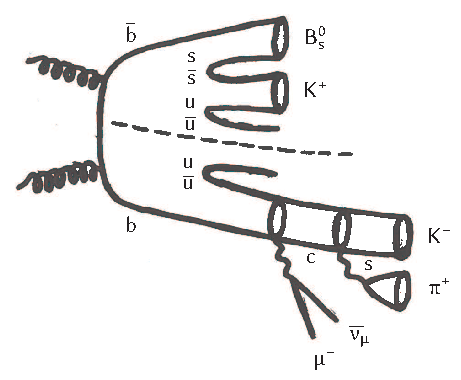
\includegraphics{graphics/intro/tikz/tagging}
  \caption{Production and decay mechanisms exploited by flavour-tagging algorithms.
           Same-side tagging determines the flavour of the $\Bs$ or $\Bsbar$ meson from the charge of the kaon that is produced close to it
           (top half of the figure).
           Opposite-side tagging determines the flavour from the charges of the decay products of the ``opposite'' b or $\qbar[b]$ quark in
           the event
           (bottom half of the figure).}
  \label{fig:tagging}
\end{figure}

The charge of the beauty quark on the ``opposite side of the event'' can be determined from the charges of the electron, muon, or kaon in
the decay of the hadron it formed. This procedure is termed \emph{opposite-side tagging} and is described in
reference~\cite{LHCb-PAPER-2011-027}.

The efficiency of opposite-side tagging is limited. The required charged particles are produced in many, but not all beauty decays. In
addition, the decay products may not be detectable by the LHCb detector. There is also a probability that the determined flavour is wrong.
A neutral beauty meson may convert into its antiparticle before it decays, which gives the opposite tag. A background of charged particles
from elsewhere in the event gives additional wrong tags. The resulting effective fraction of $\Bs$ mesons with a correct opposite-side tag
in the \BstoJpsiKK{} measurement is 2.6\% (see Section~\ref{sec:ana_tagging}).

When combined with an (anti)up quark, the remaining quark from the s$\qbar[s]$ pair forms a charged kaon. In \emph{same-side kaon tagging}
the flavour of the $\Bs$ meson is estimated by determination of the charges of kaons that are close to it in momentum
space~\cite{LHCb-CONF-2012-033}. This procedure is limited by other possibilities for fragmentation and hadronization of the strange quark
and by detection of the correct kaon. The effective fraction of $\Bs$ mesons with a correct same-side tag is 1.3\% in the \BstoJpsiKK{}
measurement.


%%%%%%%%%%%%%%%%%%%%%%%%%%%%%%%%%%%%%%%%%%%%%%%%%%%%%%%%%%%%%%%%%%%%%%%%
\subsection{\texorpdfstring{\BstoJpsiKK}{Bs0->J/psi K+K-} Decays in LHCb}
\label{subsec:intro_LHCb_Jpsiphi}
%%%%%%%%%%%%%%%%%%%%%%%%%%%%%%%%%%%%%%%%%%%%%%%%%%%%%%%%%%%%%%%%%%%%%%%%

LHCb is one of the four large experiments that analyse the particles produced by LHC collisions. The LHCb detector measures particle
trajectories in the ``forward'' direction, that is, along the direction of one of the proton beams. Particles produced with momenta at
angles between typically 1 and 15 degrees from the beam direction can be detected. Although this \emph{acceptance region} covers only a
small part of possible particle directions, it contains roughly a quarter of all produced beauty quarks. This makes the LHCb design
efficient for studies of hadrons containing beauty quarks.

The particles that are produced in an LHC collision get a momentum from the boost introduced by asymmetric parton momenta, but also from
the centre-of-mass energy that is available in the parton interaction. $\Bs$ mesons that are selected for the analysis of \BstoJpsiKK{}
decays have an average momentum of the order of a hundred \GeVc{} (see Figure~\ref{fig:introHists_BMomentum}). With the 5.4\unitsp\GeV{}
$\Bs$-meson mass~\cite{PDG}, this gives an average Lorentz factor of about 20.

The $\Bs$ meson has a relatively large mean lifetime of about 1.5\unitsp{}ps \cite{Amhis:2012bh}. As a result of the significant lifetime
and boost, $\Bs$ mesons cover a typical distance of several millimetres before they decay. The measurement of this \emph{flight distance}
is used to infer the decay time. It is determined by reconstructing the positions of the points of production and decay. The measured
distribution for $\Bs$ mesons that are used in the \BstoJpsiKK{} measurement is shown in Figure~\ref{fig:introHists_flightDist}.

\begin{figure}[tbhp]
  \centering
  \begin{subfigure}{0.497\textwidth}
    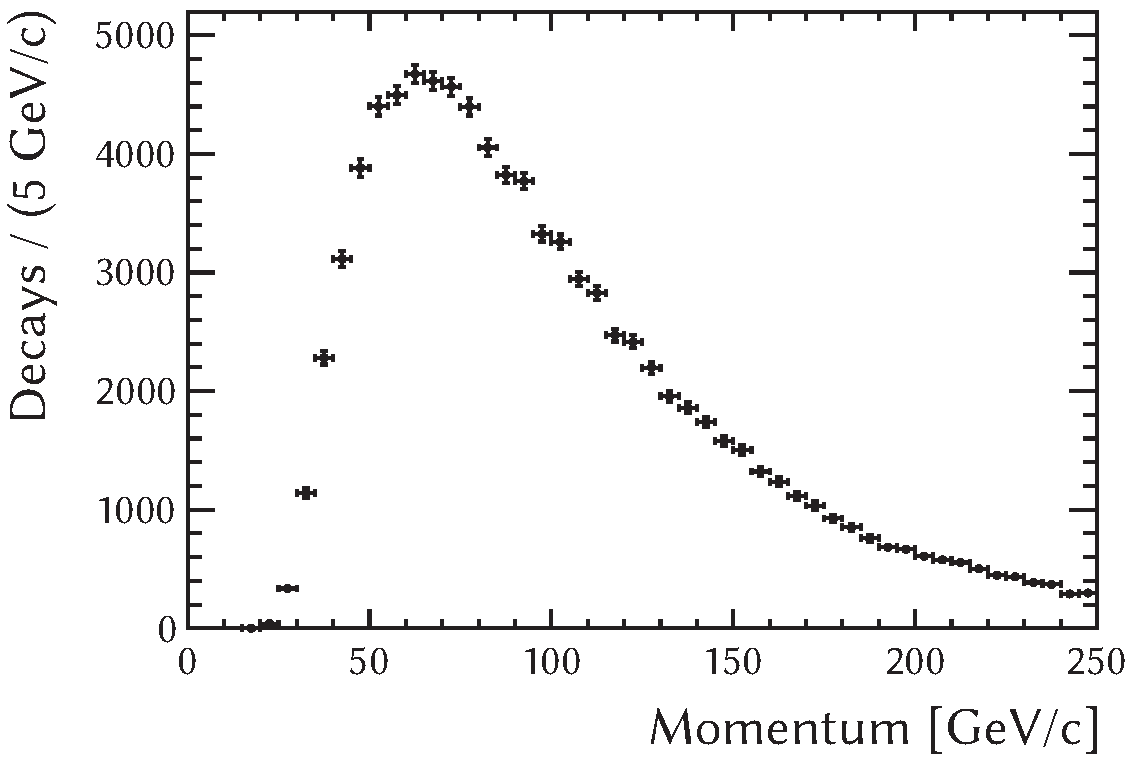
\includegraphics[width=\textwidth]{graphics/intro/BMomentum}
    \caption{}
    \label{fig:introHists_BMomentum}
  \end{subfigure}%
  \hfill%
  \begin{subfigure}{0.497\textwidth}
    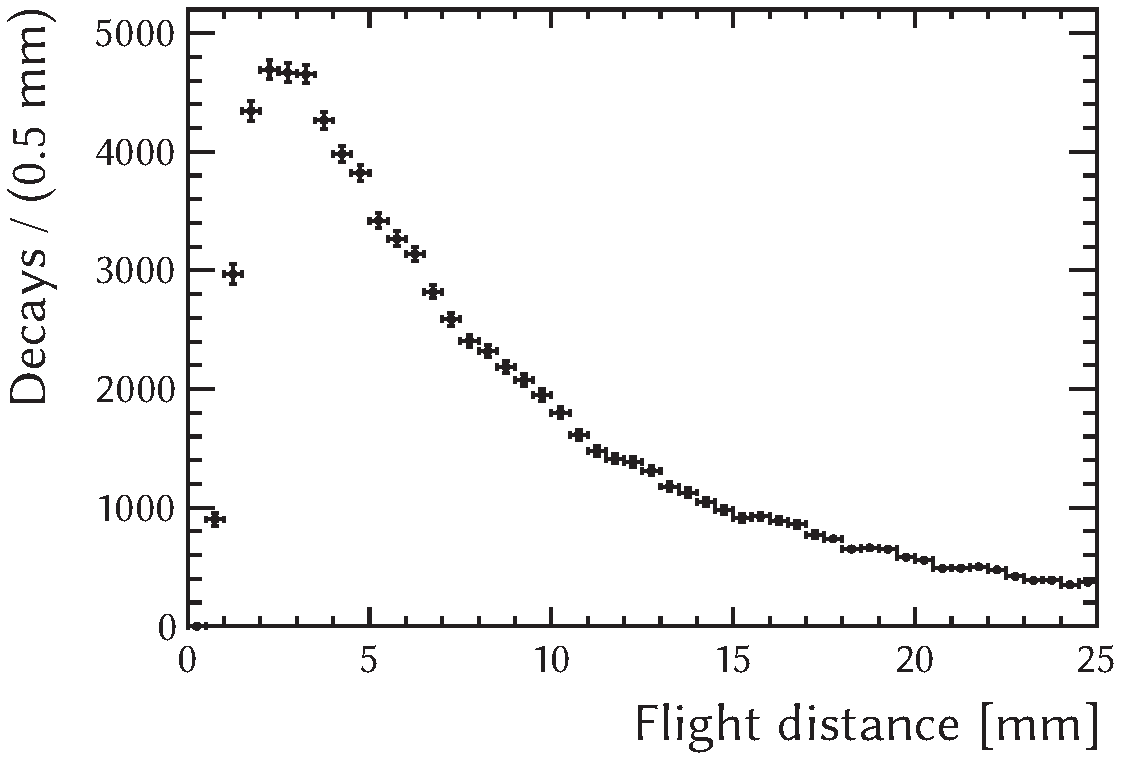
\includegraphics[width=\textwidth]{graphics/intro/flightDist}
    \caption{}
    \label{fig:introHists_flightDist}
  \end{subfigure}
  \caption{Histograms of (a) the reconstructed momenta and (b) the flight distance of $\Bs$ mesons in the \BstoJpsiKK{} measurement.}
  \label{fig:introHists}
\end{figure}

Since LHC bunches have a finite size and the positions of the colliding protons in their respective bunches are not known a priori, the
interaction point has to be measured for each collision. This is done by measuring the trajectories of produced particles and extrapolating
them to the point of their common origin. This point is termed the \emph{primary vertex}. The \emph{secondary vertex} is the point where
the $\Bs$ decayed, which is measured with only the trajectories of the four decay $\Bs$ products.

Figure~\ref{fig:vertices} schematically shows the vertices in the \BstoJpsiKK{} decay. The vertices are depicted by ellipsoids with a size
that represents the uncertainty in the vertex position. The resolution on the vertex position is better for the primary vertex than for the
secondary vertex, because a larger number of particles is available for the reconstruction of the former.

The secondary vertex is constructed from the $\mumu$ vertex and the $\KK$ vertex, where the former dominates because of a better
resolution. This is caused by the fact that only $\KK$ invariant masses in a range between 0.99 and 1.05~\GeV{} are selected, which is just
above the threshold of twice the kaon mass. As a result, the opening angle between the $\Kp$ and $\Km$ trajectories is small, which gives
the measurement of the point of common origin a large uncertainty.

\begin{figure}[htb]
  \centering
  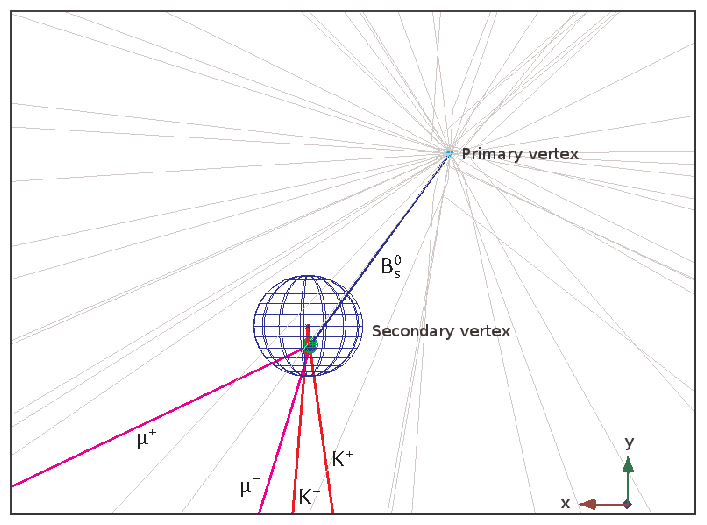
\includegraphics{graphics/intro/tikz/vertices}
  \caption{Vertices in a \BstoJpsiKK{} decay \cite{vanEijk:2012}.
           The vertices are indicated by ellipsoids with a size that represents the uncertainty in the vertex position.
           The primary vertex is indicated by the cyan ellipsoid, the $\mumu$ vertex with the small green ellipsoid
           and the $\KK$ vertex with the large blue ellipsoid.
           The secondary vertex is the combination of the $\mumu$ and $\KK$ vertices.}
  \label{fig:vertices}
\end{figure}

The decay time can be calculated from the flight distance, provided that also the $\Bs$ momentum is known:
\begin{equation}
  \label{eq:decayTime}
  t = \frac{1}{\gamma(v)}\,\frac{d}{v} = \frac{m d}{\gamma(v) m v} = \frac{m d}{|\vec{p}|} \ \ ,
\end{equation}
where $t$ is the decay time in the rest system of the $\Bs$, $d$ the flight distance, $v$ the $\Bs$ velocity, $\gamma$ the
corresponding Lorentz factor, $\vec{p}$ the momentum, and $m$ the $\Bs$ mass. The momentum is reconstructed as a vector sum of the
decay-product momenta, which are also required to calculate the decay angles. Momenta of charged particles are inferred from the curvature
of their tracks in the magnetic field of the detector.

The $\Bs$ momentum and flight distance are estimated by combining information from measured particle momenta and extrapolated
positions~\cite{Hulsbergen:2005pu}. Uncertainties in the measurements are propagated and ultimately lead to an uncertainty in the estimated
decay time. This decay-time resolution is estimated for each $\Bs$ decay and taken into account in the analysis (see
Section~\ref{subsec:ana_time_res}). The effective resolution is about 0.05\unitsp{}ps. This suffices to resolve the oscillations in the
\BstoJpsiKK{} decay-time distribution, which have a period of 2π/$\Dms$\textapprox0.35\unitsp{}ps.

Before the vertex positions and momenta can be determined, the four particles from a \BstoJpsiKK{} decay have to be selected from all
particles that are produced in an LHC event. Since the particle multiplicity in inelastic proton--proton collisions is high, there is a
significant probability to select four particles that do not originate from a $\Bs$ decay.

Combinations of four particles that are considered for analysis are called \emph{decay candidates}. Candidates can either be real
\BstoJpsiKK{} decays (\emph{signal}) or combinations that fake the decay signature (\emph{background}). Distributions of decay time and
decay angles for background events are subtracted from the measured distributions to obtain the net signal contribution (see
Section~\ref{sec:ana_bkgSub}).

There are several categories of background decay candidates. Most background is \emph{combinatorial}, which means that candidates are
formed from random combinations of four particles. Often all four particles originate directly from a primary vertex. This combinatorial
background is called \emph{prompt}. For non-prompt candidates some of the particles originate from a secondary vertex in the decay of a
long-lived particle, for example a beauty hadron. Since the $\mumu$ vertex has a relatively small uncertainty in comparison with the $\KK$
vertex, this often involves a $\Jpsi\to\mumu$ decay combined with kaons from the primary vertex.

To reduce the amount of prompt background that is considered for further analysis, candidates for which the secondary vertex is too close
to the primary vertex are rejected. This leads to a detection inefficiency for candidates with a small flight distance and, consequently,
small decay time. This effect is visible in Figure~\ref{fig:introHists_flightDist}, where the number of decays goes to zero at small decay
time.

Another background category is \emph{misidentified background}, which comprises decays where one or more particles have been incorrectly
identified.  The two misidentified backgrounds that are taken into account in the \BstoJpsiKK{} measurement are \BdtoJpsiKstKpi{} and
\LbtoJpsipK. In the $\Bd$ decay the pion is misidentified as a kaon and in the $\Lb$ decay the proton as a kaon.

There are different stages of event and decay-candidate selection. Each stage is optimized to find signal decays with high efficiency and
at the same time keep the background at a manageable level. The first three selection stages are \emph{triggers} \cite{LHCb-DP-2012-004},
which are designed to select events of interest \emph{online}, before detector data are stored for further analysis. Two \emph{offline}
stages select decay candidates in the stored events.

The first trigger is called \emph{Level 0} (L0). It is implemented in the detector hardware and designed to bring the rate of incoming
events down to less than 1\unitsp{}MHz, which is the maximum frequency at which the detector can be read out. In proton collisions that
create beauty hadrons, particles are created in all directions in the centre-of-mass frame of the parton interaction. As a result,
particles in these collisions typically have significant momentum components in the direction transverse to the proton beams. This is used
by the L0 trigger, which selects only events that contain particles above a transverse-momentum threshold.

Events that are selected by L0 are processed by the \emph{High Level Trigger} (HLT). This trigger is implemented in software and consists
of two stages: HLT1 and HLT2. In the first stage a minimal reconstruction of particle trajectories and vertices is performed. For the
\BstoJpsimumuKK{} measurement, events are selected if they contain the signatures of the muons in this decay.

HLT1 selects roughly 40\unitsp{}kHz of events, which are subsequently processed by HLT2. At this stage a more complete particle
reconstruction is performed. Events are selected for the \BstoJpsiKK{} measurement if they contain $\mumu$ pairs that are compatible with a
$\Jpsi$ decay at a significant distance from a primary vertex. Events for all LHCb measurements are stored at a rate of 3--5\unitsp{}kHz.

The first stage of the offline selection fully reconstructs the particle trajectories and vertices in the remaining events and selects
combinations of muon and kaon pairs that form \BstoJpsiKK{} candidates. A set of loose selection criteria is applied to filter out
part of the background, which reduces the number of remaining candidates to a manageable level. This procedure is termed \emph{stripping}.

Stripping yields about twelve million \BstoJpsiKK{} decay candidates for 2011 and 2012. A second set of stricter offline selection criteria
is applied, optimized to find the best compromise between selecting as many signal and as few background candidates as possible. At this
stage about 230 thousand candidates are retained for further analysis, of which roughly 40\% is signal (see Section~\ref{sec:ana_bkgSub}).

The total set of selection requirements for particles and decay candidates removes background, but also a significant part of the signal.
%This can be seen in the flight-distance distribution of Figure~\ref{fig:introHists_flightDist}. The original decay-time distribution has
%approximately an exponential shape. Since the decay time and $\Bs$ momentum are uncorrelated, also an exponential shape is expected for the
%flight-distance distribution. The lack of entries at small flight distance is a result of the selection inefficiency.
Since the efficiency of the selection depends on the decay time and the decay angles, the observed distributions of these variables do not
directly reflect the underlying true distributions. This effect has to be taken into account in the model of the decay (see
Sections~\ref{subsec:ana_time_acc} and \ref{sec:ana_angles}).


%%%%%%%%%%%%%%%%%%%%%%%%%%%%%%%%%%
\subsection{The LHCb Detector}
\label{subsec:intro_LHCb_detector}
%%%%%%%%%%%%%%%%%%%%%%%%%%%%%%%%%%

\begin{figure}[ptb]
  \centering
  \begin{subfigure}{0.78\textwidth}
    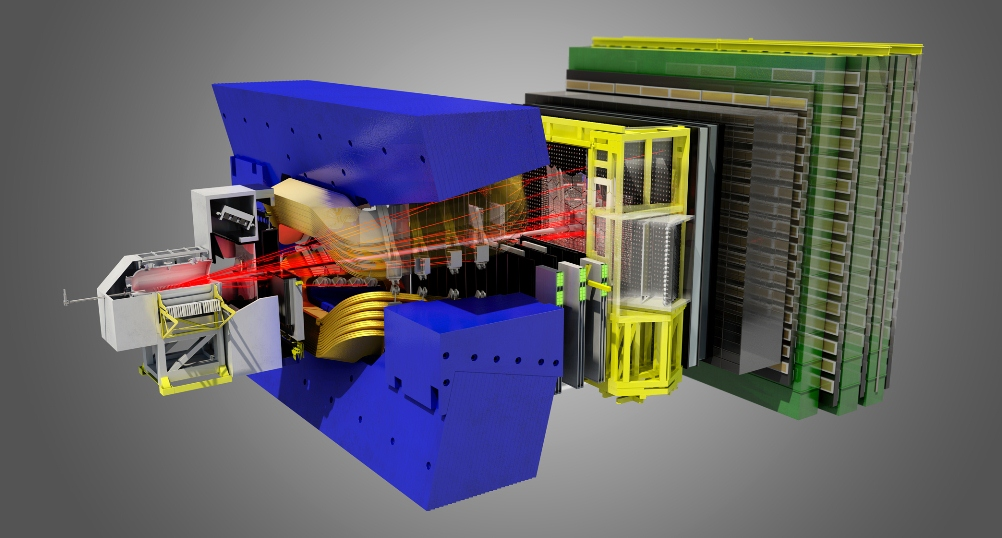
\includegraphics[width=\textwidth]{graphics/intro/detector_3D.jpg}
    \caption{}
    \label{fig:LHCb_3D}
  \end{subfigure}

  \vspace*{0.03\textwidth}
  \begin{subfigure}{\textwidth}
    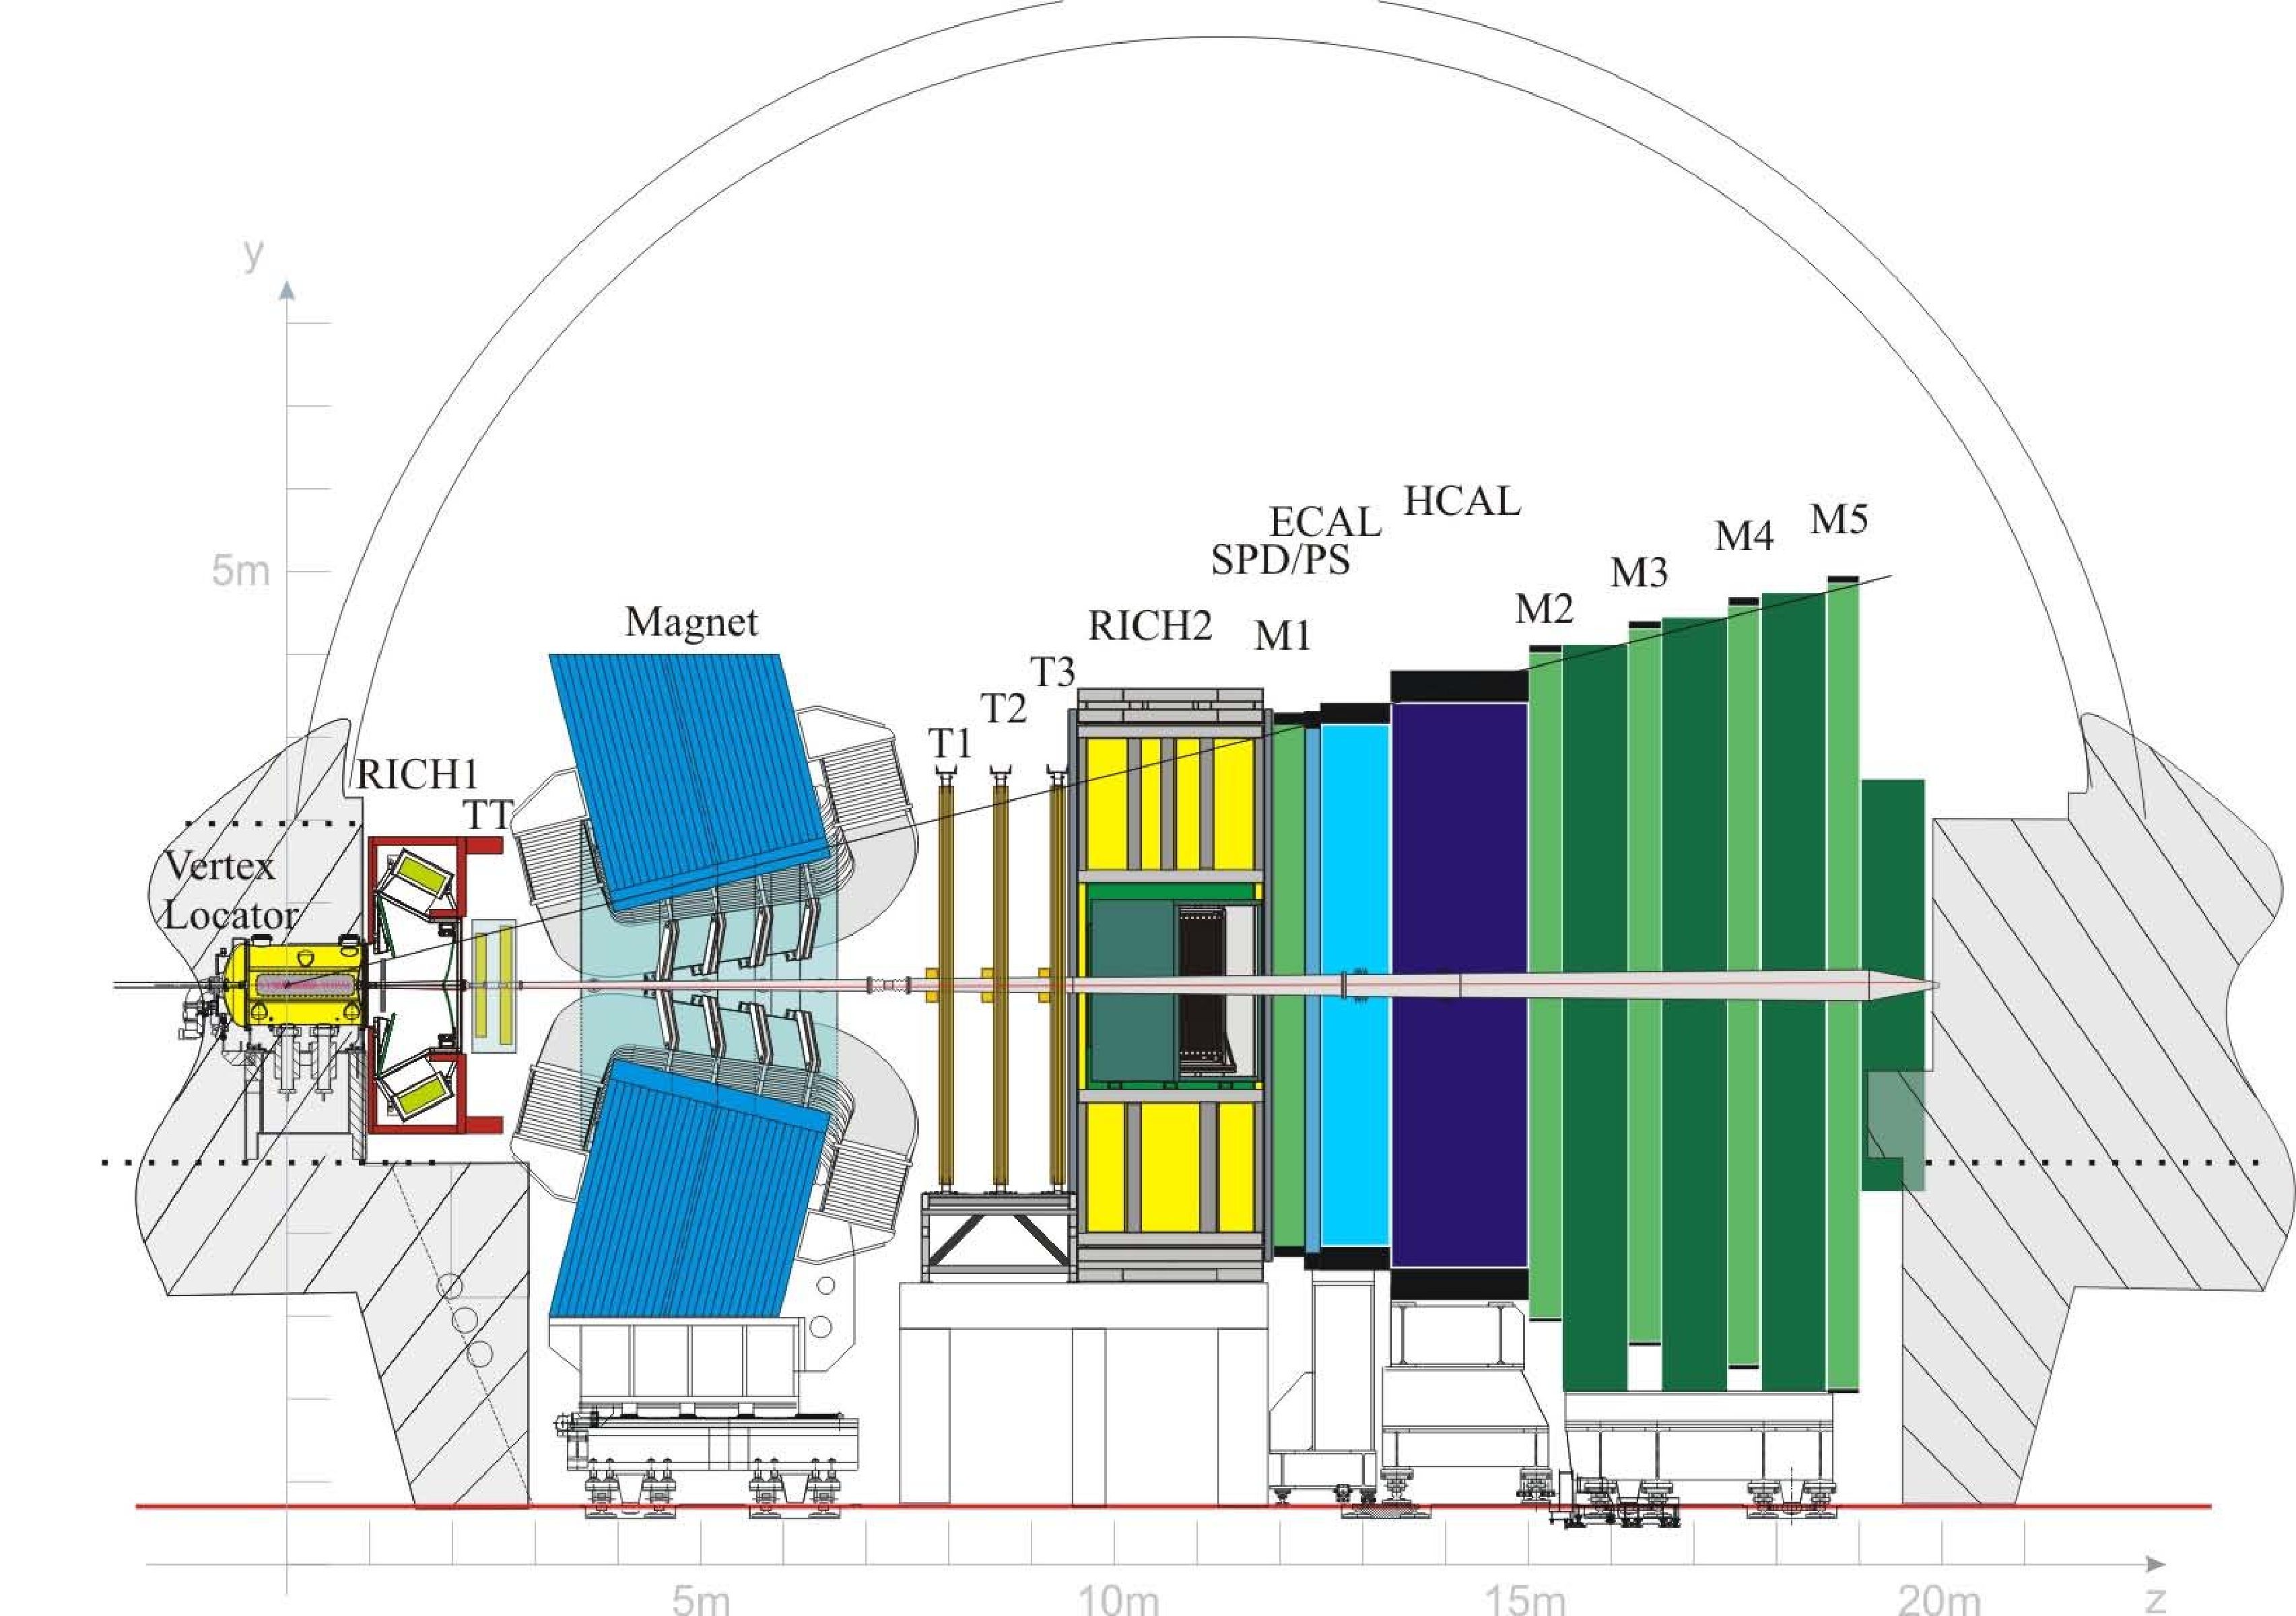
\includegraphics[width=\textwidth]{graphics/intro/detector_cross}
    \caption{}
    \label{fig:LHCb_cross}
  \end{subfigure}

  \caption{Schematic views of the LHCb detector.
           (a) Three-dimensional view, where particles from the proton--proton collision are depicted by red lines.
           (b) Cross sectional view of the various subdetectors, which are discussed in the text.}
  \label{fig:LHCb}
\end{figure}

The LHCb detector was mainly built to measure beauty- and strange-hadron decays into particles with an electric charge. It is capable of
measuring charged-particle trajectories and the locations of primary and secondary vertices with a precision that is good enough to resolve
oscillations in decay-time distributions with a frequency $\Dms$\textapprox18\unitsp{}ps. Another important feature of the detector is its
ability to identify different types of particles.

The detector and its performance are described in detail in references~\cite{Alves:2008zz} and \cite{LHCb-DP-2014-002}. A schematic view is
shown in Figure~\ref{fig:LHCb}. The subdetectors are placed around the LHC beams, which come in from the left and right. The interaction
point is contained within the subdetector labelled ``Vertex Locator'' on the left of Figure~\ref{fig:LHCb_cross}. Particles that are
produced within the LHCb acceptance region traverse the various subdetectors from the left to the right. This is indicated by the red lines
in Figure~\ref{fig:LHCb_3D}.

A magnetic field with an integrated strength of 4\unitsp{}Tm is produced by a dipole magnet between approximately 3 and 8\unitsp{}m from
the interaction point. The saddle-shaped coils of the magnet are surrounded by the magnet yoke, which is indicated by the blue block in
Figure~\ref{fig:LHCb}. The magnetic field is pointing either upwards or downwards, bending charged-particle trajectories in the horizontal
plane. During the two years of LHC running, the direction of the magnetic field was reversed several times to control systematic
uncertainties related to the measurement of particle trajectories.

Trajectories of charged particles are reconstructed by measurement of the positions at which the particles traverse the various
\emph{tracking detectors} of LHCb. These measurements are all based on electromagnetic interactions of the particle with detector material.
The signal from a particle interaction with sensitive detector material is called a \emph{hit}. The collection of hits that represent the
trajectory of a particle is a \emph{track}.

The LHCb tracking system consists of four components. The \emph{Vertex Locator} (\velo) and the \emph{Tracker Turicensis} (TT)
before the magnet and the \emph{Inner Tracker} (IT) and \emph{Outer Tracker} (OT) behind the magnet. Together, the IT and OT form the
three tracking stations labelled by ``T1'', ``T2'', and ``T3'' in Figure~\ref{fig:LHCb_cross}. The inner region of roughly
0.5\unitsp{}m\textsuperscript{2} around the proton beams is covered by the IT and the region up to approximately 3\unitsp{}m from the beams
by the OT.

Hit information from all tracking detectors is combined to build tracks. The momentum of a particle can be inferred from the radius of
curvature of the track in the magnetic field, given the charge of the particle. Since most charged particles that live long enough to reach
the detector are electrons, muons, pions, kaons, and protons, a unit charge can be assumed. The sign of the charge is determined from the
direction of the track curvature.

The performance of the tracking system is shown in Figures~\ref{fig:detPerf_momRes} and \ref{fig:detPerf_massRes}. The former figure shows
the relative resolution of the momentum measurement for muon tracks in $\Jpsi\to\mumu$ decays, which varies from roughly 0.5\% to 1.1\% as
a function of momentum over a range of 2 to 300~\GeVc. The resulting resolution of the dimuon invariant-mass measurement is shown in the
latter figure. The relative mass resolution is about 0.5\% up to 10\unitsp\GeV, but increases to 1.9\% at the $\Zz$ mass.
\begin{figure}[ptb]
  \begin{subfigure}{0.49\textwidth}
    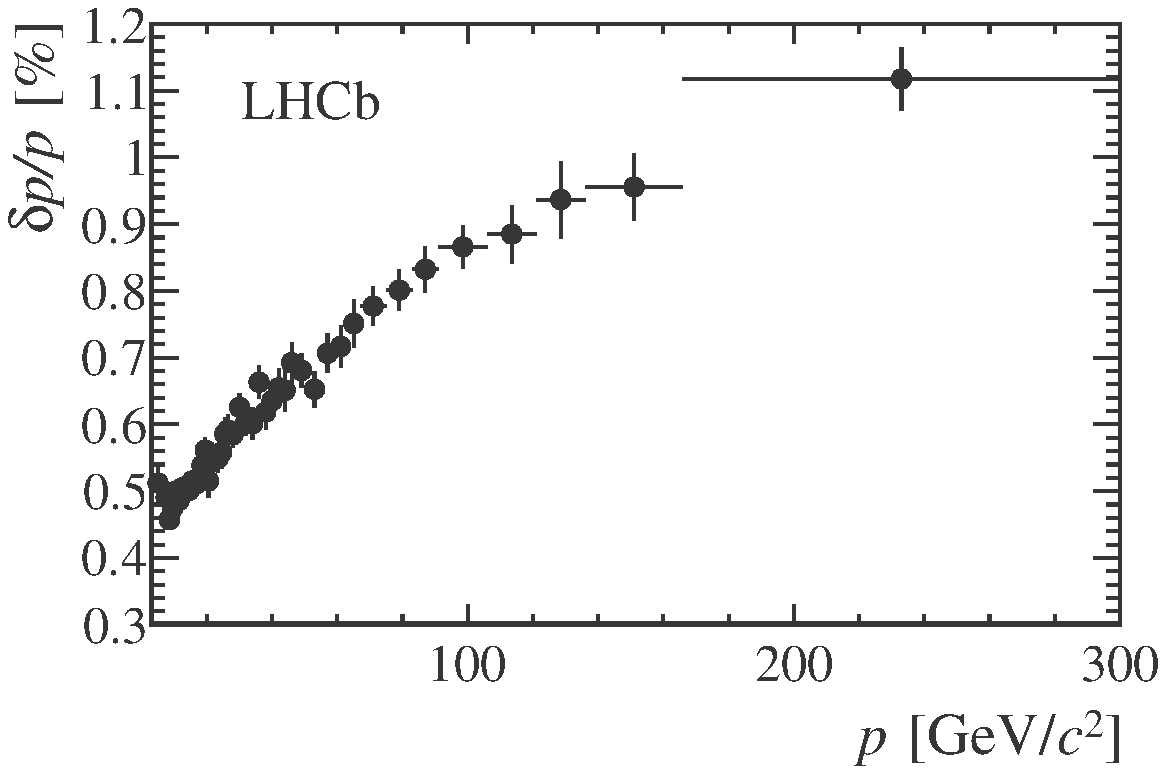
\includegraphics[width=\textwidth]{graphics/intro/dppVsp-crop-cmyk}
    \caption{}
    \label{fig:detPerf_momRes}
  \end{subfigure}%
  \hfill%
  \begin{subfigure}{0.49\textwidth}
    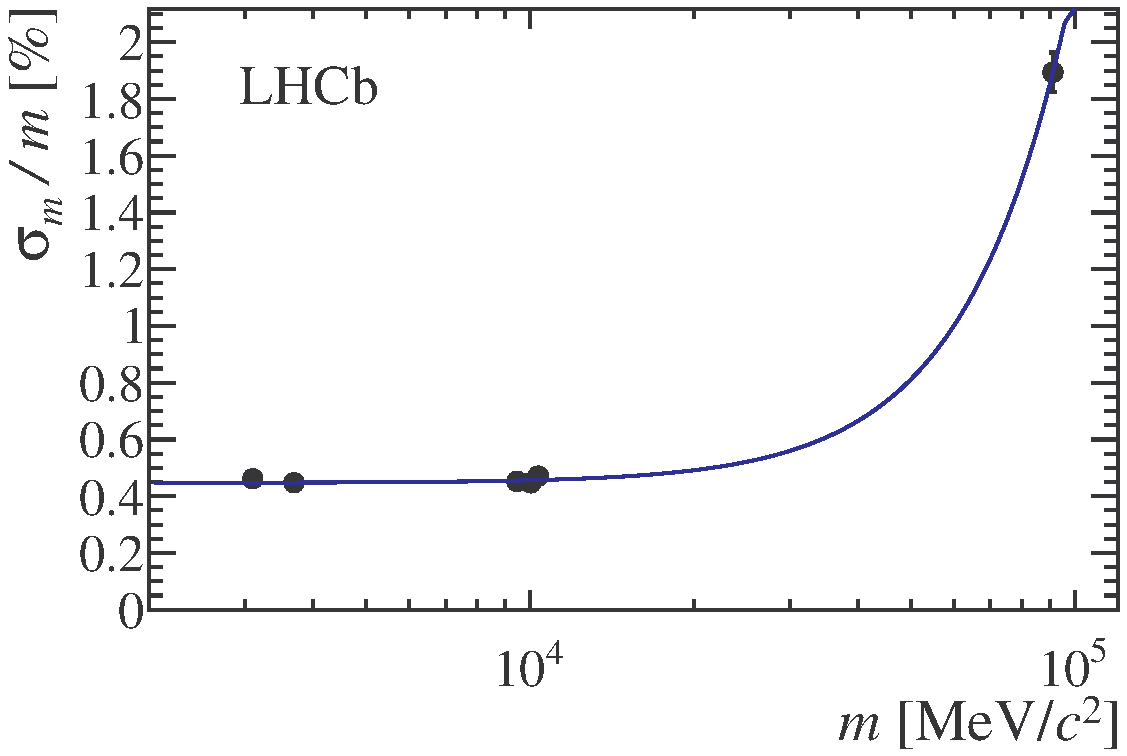
\includegraphics[width=\textwidth]{graphics/intro/relResolutionVsMass-crop-cmyk}
    \caption{}
    \label{fig:detPerf_massRes}
  \end{subfigure} \\

  \vspace*{0.01\textwidth}

  \begin{subfigure}{0.49\textwidth}
    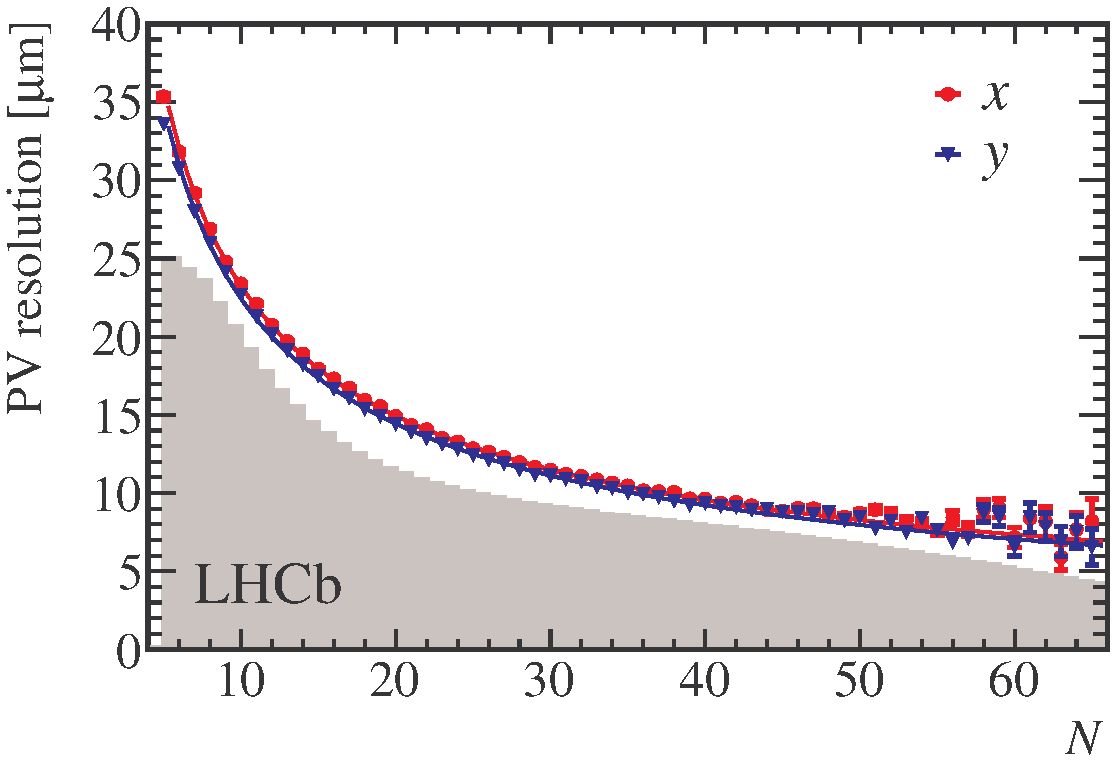
\includegraphics[width=\textwidth]{graphics/intro/DataResXY_1PV_2012-crop-cmyk}
    \caption{}
    \label{fig:detPerf_vertRes}
  \end{subfigure}%
  \hfill%
  \begin{subfigure}{0.49\textwidth}
    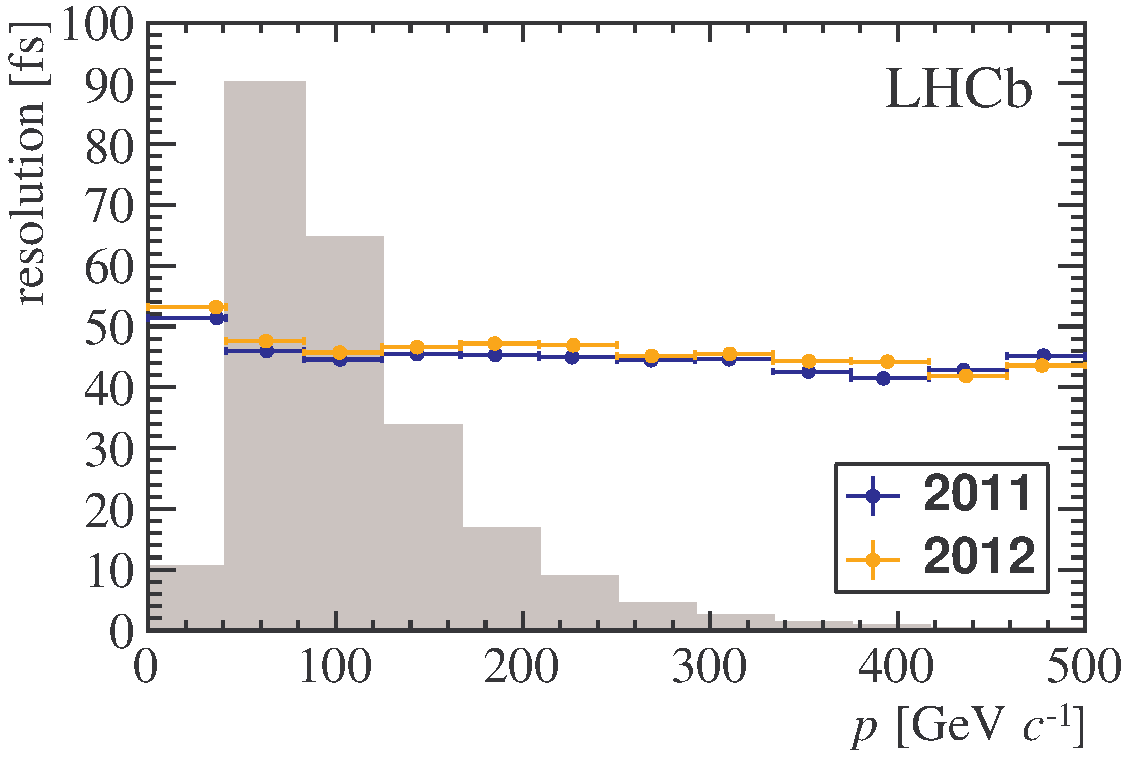
\includegraphics[width=\textwidth]{graphics/intro/decaytimeresoVsMomentumJPsiPhi-crop-cmyk}
    \caption{}
    \label{fig:detPerf_timeRes}
  \end{subfigure}

  \caption{Performance of the LHCb detector~\cite{LHCb-DP-2014-002}.
           (a) Relative momentum resolution as a function of momentum for muon tracks in $\Jpsi\to\mumu$ events.
           (b) Relative $\mumu$ invariant-mass resolution as a function of mass,
               measured for the $\Jpsi$, $\psitwoS$, $\upsS[1]$, $\upsS[2]$, $\upsS[3]$, and $\Zz$ resonances.
           (c) Primary vertex resolution as a function of the number of tracks in the vertex,
               separately for the two directions in the plane transverse to the beam direction.
           (d) Decay-time resolution of prompt \BstomumuKK{} background as a function of the combined $\mumu\,\KK$ momentum,
               separately for 2011 and 2012.}
  \label{fig:detPerf}
\end{figure}

Vertices are reconstructed by extrapolating tracks to the point where they are closest together. The most precise information on vertex
locations comes from the \velo, which detects particles very close to the interaction point down to a radius of 8\unitsp{}mm
around the beams.

Figure~\ref{fig:detPerf_vertRes} shows the resolution of primary vertices in LHCb as a function of the number of tracks originating from
the vertex. A minimum of five tracks is required, where the resolution is about 35\unitsp\micron. The resolution improves with the number
of tracks to less than 10\unitsp\micron{} for more than 40 tracks.

Since only four tracks originate from the secondary vertex, its resolution dominates the uncertainty of the decay-time measurement. For
\BstomumuKK{} events the decay-time resolution is measured with prompt background, for which the true decay time is equal to zero (see
Section~\ref{subsec:ana_time_res}). The resulting resolution as a function of $\mumu\,\KK$ momentum is shown in
Figure~\ref{fig:detPerf_timeRes}. Its value varies between roughly 0.04\unitsp{}ps and 0.05\unitsp{}ps.

Particles are identified with other subsystems. Electrons produce signals in the \emph{Scintillator Pad Detector} (SPD), \emph{Preshower
detector} (PS) and the \emph{Electromagnetic Calorimeter} (\ecal). The electron energy is absorbed by these detectors and no signal is
produced in the \emph{Hadronic Calorimeter} (\hcal). Pions, kaons, and protons predominantly lose energy in the \hcal{} and less in the
\ecal. Energy measurements from the calorimeters are also used in the L0 trigger to select events with high-energy particles in the
transverse direction.

Muons do not lose significant energy in the \hcal, therefore make it through the calorimeters, and produce hits in the four \emph{muon
stations} behind the \hcal{} (M2--M5 in Figure~\ref{fig:LHCb_cross}). These features distinguish muons from hadrons. The \emph{Muon System}
is completed by the station M1 before the calorimeters to provide an optimal momentum estimate for muons.

Two \emph{Ring Imaging Cherenkov} (\rich) detectors are used to distinguish the different charged hadrons. The first \rich{} detector
(\rich1) is located between the \velo{} and the magnet and the other (\rich2) behind the IT/OT. These detectors determine the velocities of
charged particles by measuring the angle at which Cherenkov light is emitted when the particle traverses the \rich{} radiator materials.
Combined with the momentum measurement this gives an estimate of the particle mass to distinguish between pions, kaons, and protons.

Figure~\ref{fig:event} shows the information from different subdetectors for an event that contains a \BstoJpsiKK{} decay candidate. The
coloured lines show reconstructed tracks. Three tracks are combined with hits in the muons stations and represent particles that have been
identified as muons.
\begin{figure}[ptb]
  \centering
  \begin{tikzpicture}
    \node[anchor=south]{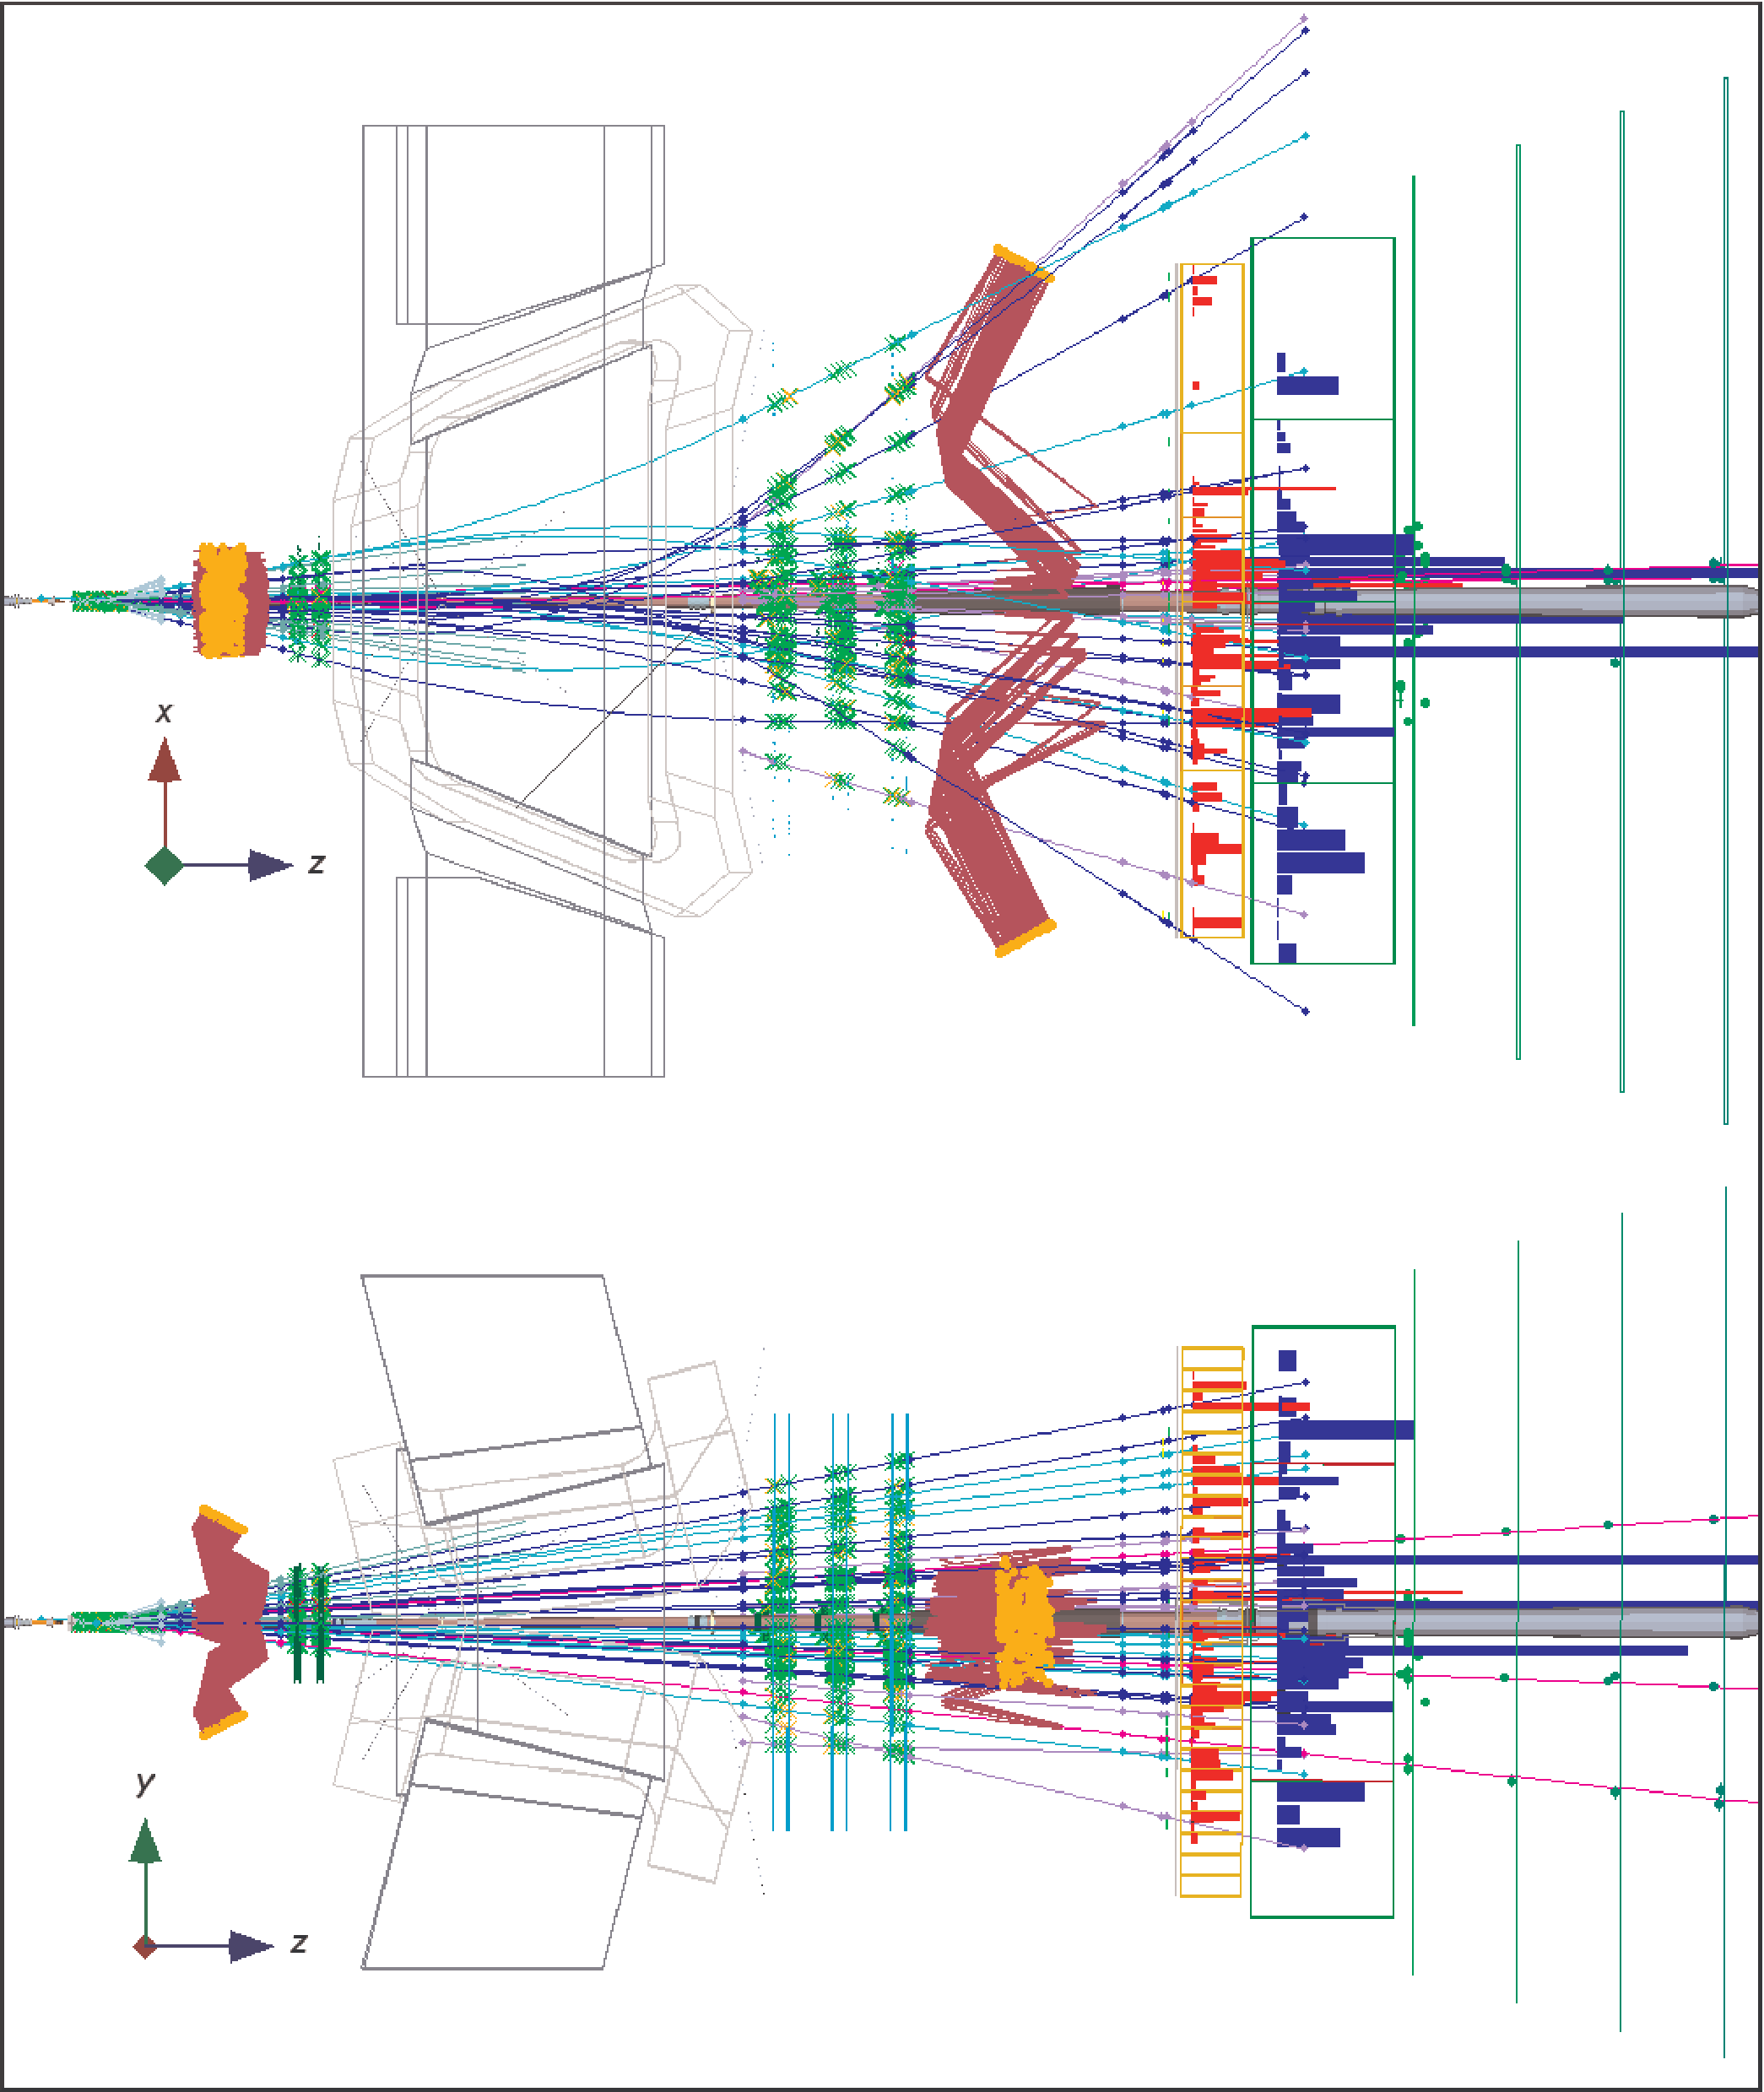
\includegraphics[width=0.95\textwidth]{graphics/intro/eventdisplay_CMYK}};
    \node at ( 0., 6.7 )  {\textbf{(a)}};
    \node at ( 0., 0.7 )  {\textbf{(b)}};
  \end{tikzpicture}
  \caption{Reconstructed particle trajectories in the LHCb detector for an event with a \BstoJpsiKK{} decay candidate \cite{vanEijk:2012}:
           (a) a view from the top and (b) a view from the side, equivalent to Figure~\ref{fig:LHCb}.
           Particle tracks are shown by the coloured lines. The green crosses indicate hits in the tracking detectors and the red and blue
           bars energy deposits in the calorimeters. Hits in the muon stations are represented by green dots. Cherenkov photons in the
           \rich{} detectors are shown by the purple lines and orange hits.}
  \label{fig:event}
\end{figure}
